\documentclass[tikz,border=4pt]{standalone}
\usepackage{amsmath}
\begin{document}
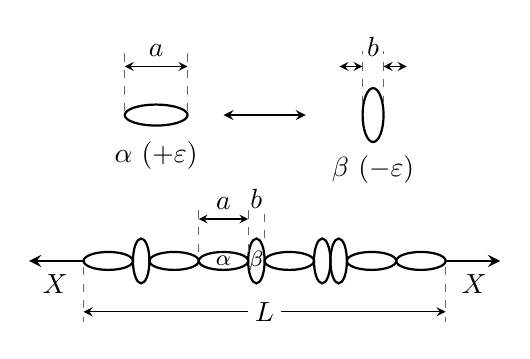
\begin{tikzpicture}[>=stealth, thick, scale=0.95]
  % Top: monomer states alpha (length a, +eps) and beta (length b, -eps)
  \begin{scope}[yshift=1.95cm]
    % State alpha: horizontal ellipse (length a = 0.85, height = 0.24)
    \draw[line width=0.8pt] (-1.45, 0) ellipse (0.42 and 0.14);
    \draw[dashed, line width=0.4pt, black!60] (-1.87, 0.05) -- (-1.87, 0.85);
    \draw[dashed, line width=0.4pt, black!60] (-1.03, 0.05) -- (-1.03, 0.85);
    \draw[<->, line width=0.45pt] (-1.87, 0.65) -- (-1.03, 0.65) node[midway, above] {$a$};
    \node[below] at (-1.45, -0.22) {$\alpha\ (+\varepsilon)$};

    % Transition arrow
    \draw[<->, line width=0.6pt] (-0.55, 0) -- (0.55, 0);

    % State beta: vertical ellipse (length b = 0.28, height = 0.68)
    \draw[line width=0.8pt] (1.45, 0) ellipse (0.14 and 0.36);
    \draw[dashed, line width=0.4pt, black!60] (1.31, 0.15) -- (1.31, 0.85);
    \draw[dashed, line width=0.4pt, black!60] (1.59, 0.15) -- (1.59, 0.85);
    \draw[<->, line width=0.45pt] (1.00, 0.65) -- (1.31, 0.65);
    \draw[<->, line width=0.45pt] (1.90, 0.65) -- (1.59, 0.65);
    \node[above] at (1.45, 0.65) {$b$};
    \node[below] at (1.45, -0.40) {$\beta\ (-\varepsilon)$};
  \end{scope}

  % Bottom: Polymer chain under tension X, total length L
  \begin{scope}[yshift=0cm]
    % Sequence: alpha, beta, alpha, alpha, beta, alpha, beta, beta, alpha, alpha
    % Widths: alpha=0.66, beta=0.22
    % Start at x = -2.42
    \def\xa{0.66}
    \def\xb{0.22}
    % Draw chain elements
    \draw[line width=0.8pt] (-2.09, 0) ellipse (0.33 and 0.12);
    \draw[line width=0.8pt] (-1.65, 0) ellipse (0.11 and 0.30);
    \draw[line width=0.8pt] (-1.21, 0) ellipse (0.33 and 0.12);
    \draw[line width=0.8pt] (-0.55, 0) ellipse (0.33 and 0.12);
    \node at (-0.55, 0) {\footnotesize $\alpha$};
    \draw[line width=0.8pt] (-0.11, 0) ellipse (0.11 and 0.30);
    \node at (-0.11, 0) {\footnotesize $\beta$};
    \draw[line width=0.8pt] (0.33, 0) ellipse (0.33 and 0.12);
    \draw[line width=0.8pt] (0.77, 0) ellipse (0.11 and 0.30);
    \draw[line width=0.8pt] (0.99, 0) ellipse (0.11 and 0.30);
    \draw[line width=0.8pt] (1.43, 0) ellipse (0.33 and 0.12);
    \draw[line width=0.8pt] (2.09, 0) ellipse (0.33 and 0.12);

    % Tension arrows X at both ends
    \draw[->, line width=0.95pt] (-2.42, 0) -- (-3.15, 0);
    \node[below] at (-2.80, -0.05) {$X$};
    \draw[->, line width=0.95pt] (2.42, 0) -- (3.15, 0);
    \node[below] at (2.80, -0.05) {$X$};

    % Dimension a and b on middle alpha, beta
    \draw[dashed, line width=0.4pt, black!60] (-0.88, 0.12) -- (-0.88, 0.72);
    \draw[dashed, line width=0.4pt, black!60] (-0.22, 0.12) -- (-0.22, 0.72);
    \draw[<->, line width=0.4pt] (-0.88, 0.56) -- (-0.22, 0.56) node[midway, above] {$a$};
    \draw[dashed, line width=0.4pt, black!60] (0.00, 0.30) -- (0.00, 0.72);
    \node[above] at (-0.11, 0.56) {$b$};

    % Total length L (split arrows so no white fill box appears in dark mode)
    \draw[dashed, line width=0.4pt, black!60] (-2.42, -0.08) -- (-2.42, -0.82);
    \draw[dashed, line width=0.4pt, black!60] (2.42, -0.08) -- (2.42, -0.82);
    \draw[<-, line width=0.45pt] (-2.42, -0.68) -- (-0.22, -0.68);
    \draw[->, line width=0.45pt] (0.22, -0.68) -- (2.42, -0.68);
    \node at (0, -0.68) {$L$};
  \end{scope}
\end{tikzpicture}
\end{document}
